%-------------------------------------------------------------------------------
\section{Eval}
\label{s:eval}
%-------------------------------------------------------------------------------

In our evaluation, we explore the following questions:
\begin{enumerate}
    \item Does the patch isolate LC from BE workloads for real applications?
    \item How much does the patch cost?
\end{enumerate}

All the graphs in this paper run on Linux version 6.14.2, the baseline version
that our patch builds on.

\subsection{Existing approaches}

We explore the currently available alternatives to \cgroups{} in Linux, and how
they work/don't.

\subsubsection{Realtime scheduling}

There already exists a way to configure tasks to be categorically distinct in a
way that Linux enforces globally: processes that run in real time have strict
priority over other processes.

Linux does this by using \textit{scheduling classes}. Each scheduling class
exists completely separately: classes maintain their own runqueues and
per-entity state; implement their own scheduling algorithms to choose from the
entities on their runqueue; and balance the load across runqueues on different
cores.

Linux isolates strictly between different scheduling classes: it only schedules
a lower scheduling class if the higher scheduling classes found nothing to run,
and each scheduling class tries to steal work from other cores before returning
that it has nothing to run --- these two checks represent the entry and exit
synchronization points. It is thereby true that if something in the Normal
scheduling class is running, it means there are no Fifo tasks waiting to run
anywhere on the machine.

This points to a possible solution: run LC in the Fifo scheduling class and BE
in Normal.\footnote{The Deadline scheduling class is not a good fit, since it
requires accurate knowledge of a processes runtime (processing time per request)
and period (when requests come in)} Fifo runs a priority scheduler: it has 99
priorities, each takes strict precedent over the one lower; within priorities
the scheduler enforces a global first-in-first-out (hence the Fifo class name),
based on when processes become runnable.

\begin{figure}[t]
    \centering
    \begin{subfigure}[t]{0.48\columnwidth}
        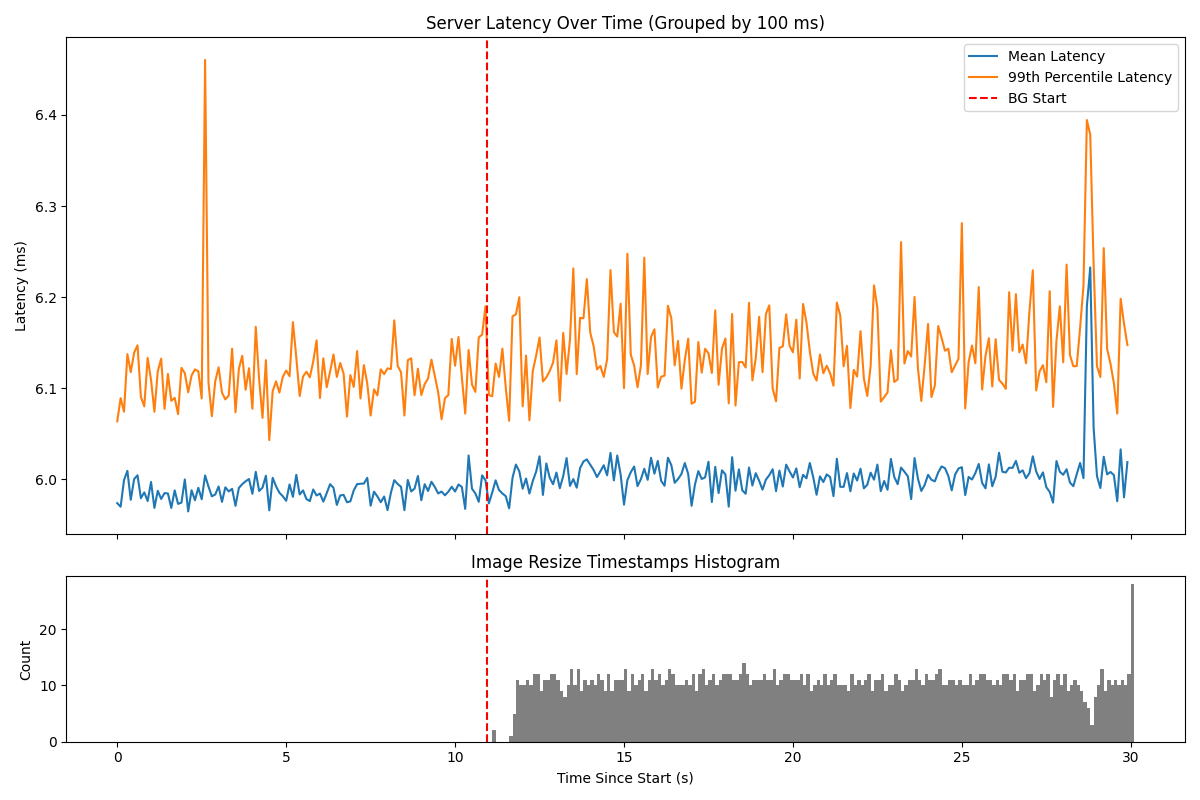
\includegraphics[width=\columnwidth]{graphs/unedited-rt-low-two.png}
        \caption{Low load}\label{fig:unedited-rt-low-two}
    \end{subfigure}
    \hspace{\fill}
    \begin{subfigure}[t]{0.48\columnwidth}
        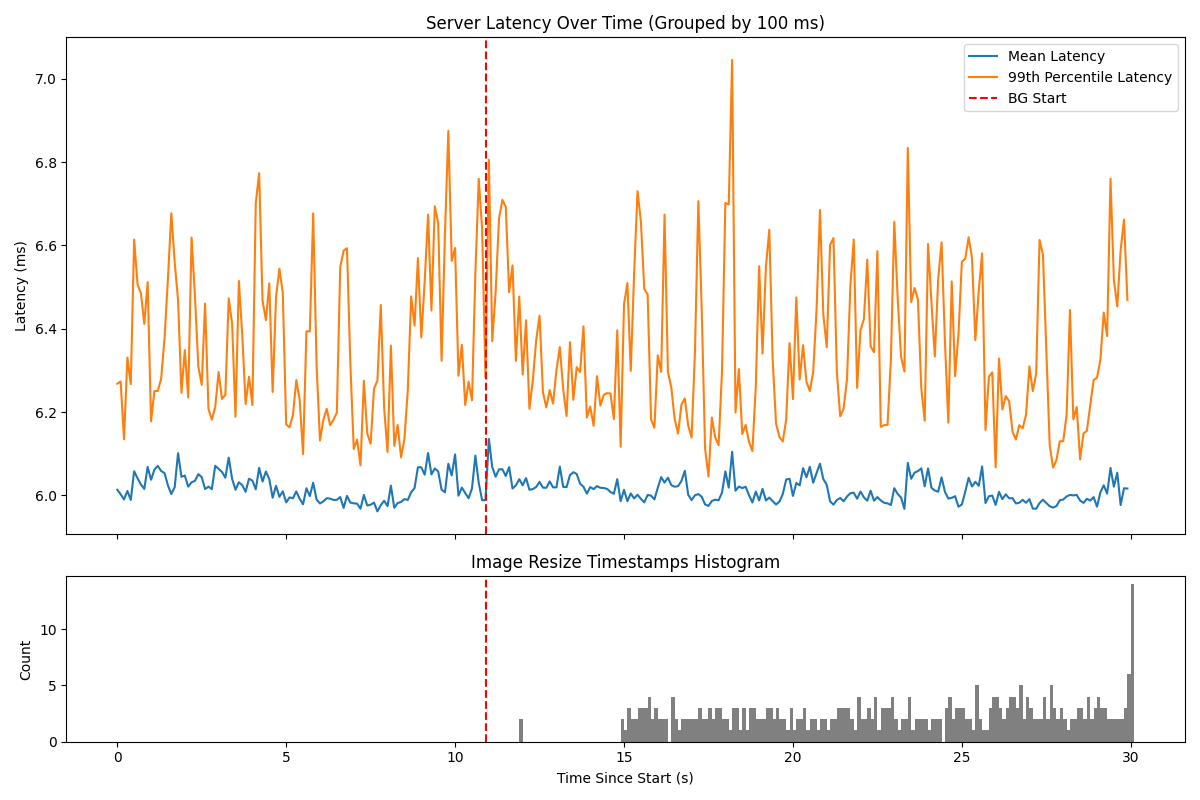
\includegraphics[width=\columnwidth]{graphs/unedited-rt-high-two.png}
        \caption{High load}\label{fig:unedited-rt-high-two}
    \end{subfigure}
    \vspace{4pt}
    \caption{Results of the same experiment, with LC running as a real time process}\label{fig:unedited-rt}
\end{figure}

We run the same experiment as in \autoref{s:intro}, but put the LC task in the
Fifo scheduling class, and leave BE tasks with the default process weight.
\autoref{fig:unedited-rt} shows the resulting measured latencies in the same low
and high load setting as previously. As expected, we see that Linux is able to
isolate the two very well. 

However, this is an untenable final solution because of Fifo's run-to-completion
scheduling, which is known to have a failure mode of head-of-line (HoL) blocking
under varied request processing times, where long-running requests monopolize
the CPU while short requests wait in the queue. The Fifo scheduler also enforces
not only cross-core isolation between different priorities, but also a global
ordering within the same priority.

The takeaway is that Linux's current mechanism of scheduling classes can isolate
workloads effectively, but existing scheduling classes use scheduling
algorithms that are not a good fit for modern workloads.

\subsubsection{\schedidle}

\schedidle{} is a scheduling \textit{policy}. Policies are not full scheduling
classes, but allow for special casing within a scheduling class. The Normal
scheduling class supports two policies: \schednormal{}, the default, and
\schedidle{}. Because both policies are in the same class the scheduler for the
Normal class is in charge of both: it keeps the tasks of both policies on the
same runqueue, and they are all scheduled using the same algorithm. Thus,
\schedidle{} is in principle not very different from just being a low-weight
process: From the scheduler's perspective, \schedidle{} entities are just
entities with a predefined low weight (currently 3).\footnote{There is,
confusingly, also an Idle scheduling \textit{class}, but that not accessible to
userspace and exists solely to manage the core's transition in and out of being
actually idle (ie running nothing).}

The main way that the Normal scheduler special-cases \schedidle{} entities from
\schednormal{} entities is during wakeup: in a 2019 patch~\cite{TODO}, Linux
added a check where, when a \schednormal{} entity becomes newly runnable, if the
core where the entity is waking up is already running something in
\schednormal{}, it will look for other cores that might be currently running a
\schedidle{} entity, and migrates the new entity there.

In doing so, Linux created a half scheduling class. In order to fully isolate
two groups of processes the scheduler needs to try synchronize across cores at
two points: entry and exit. The described patch adds only the entry check.

\schedidle{} is additionally promising because it was extended to have cgroup
support recently\cite{TODO}: a whole groups' policy can be set to \schedidle{}
via the \cgroups{} interface.

\begin{figure}[t]
    \centering
    \begin{subfigure}[t]{0.49\columnwidth}
        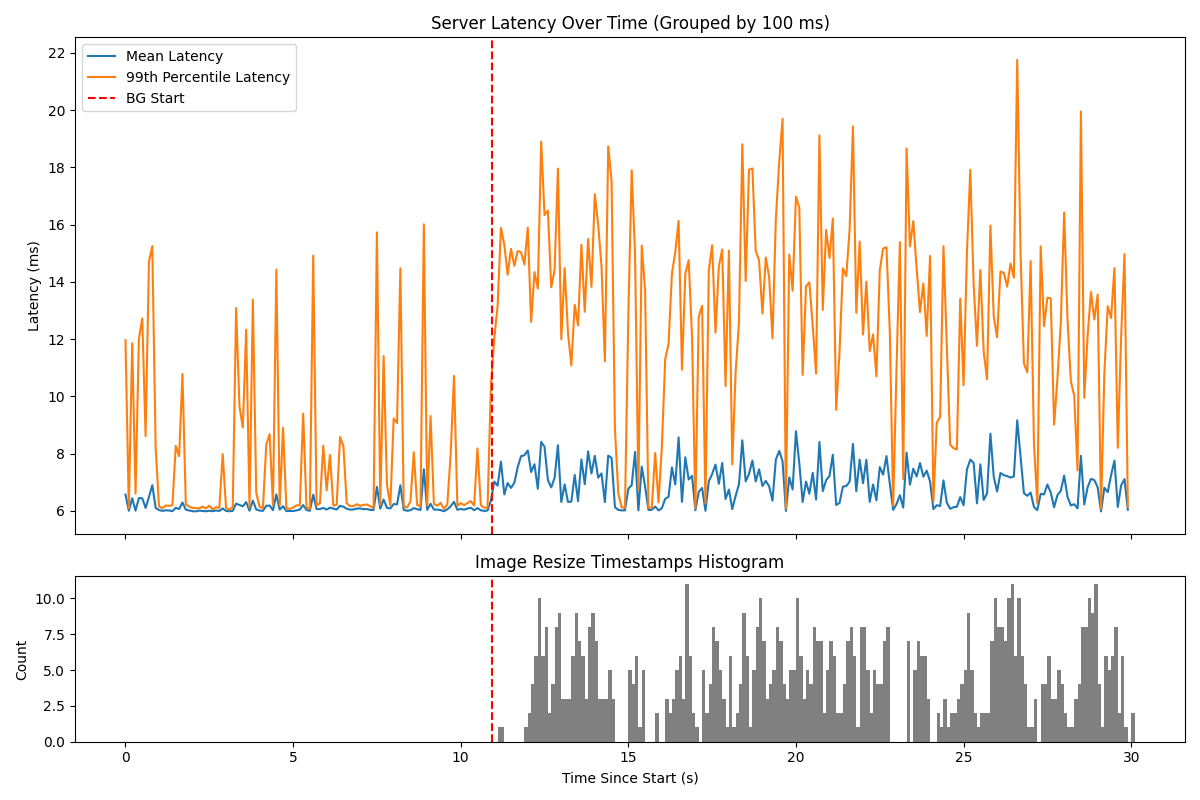
\includegraphics[width=\columnwidth]{graphs/unedited-idle-low-two.png}
        \caption{Low load}\label{fig:unedited-idle-low-two}
    \end{subfigure}
    \hspace{\fill}
    \begin{subfigure}[t]{0.49\columnwidth}
        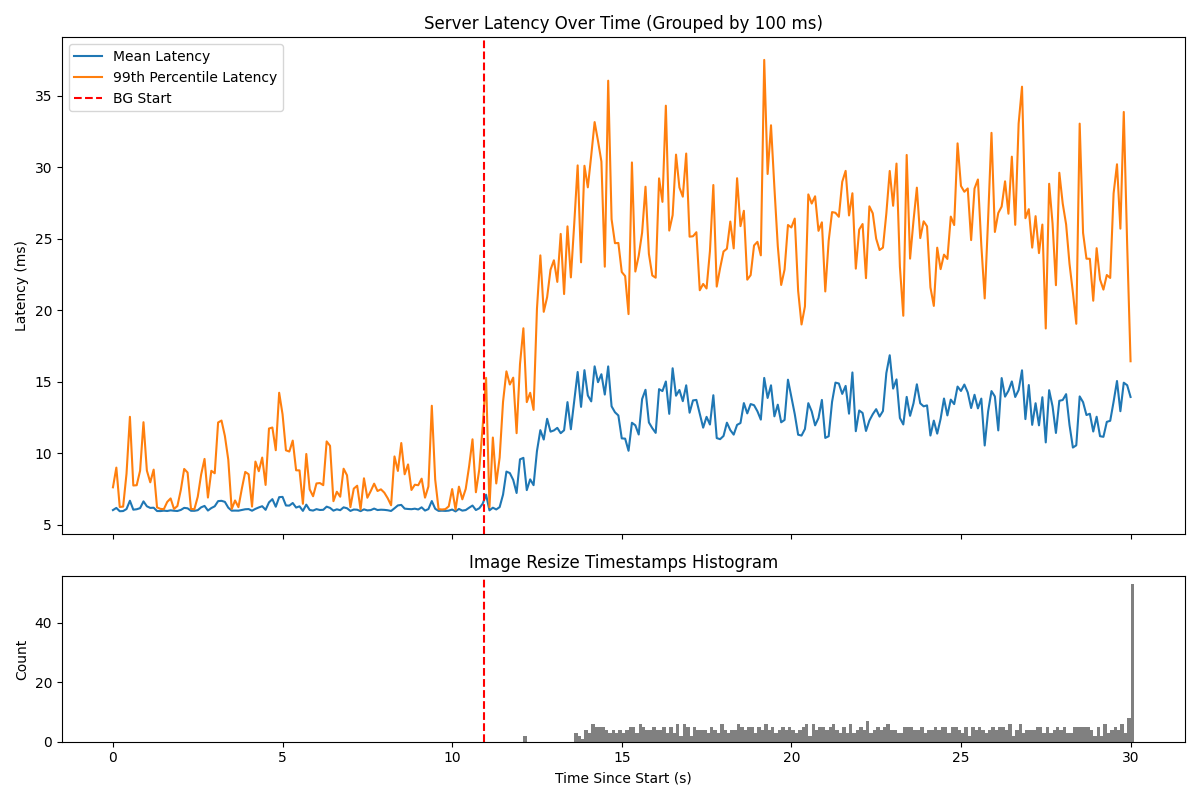
\includegraphics[width=\columnwidth]{graphs/unedited-idle-high-two.png}
        \caption{High load}\label{fig:unedited-idle-high-two}
    \end{subfigure}
    \vspace{4pt}
    \caption{using \schedidle{}}\label{fig:unedited-idle}
\end{figure}

And indeed, we find that when we use cgroups' new cpu.idle interface feature,
the latency impact of the BE tasks decreases, although it does not entirely drop
to what we saw with the Fifo class.\ \autoref{fig:unedited-idle} shows the
results, for the familiar settings of low and high load. The jump we see in the
mean latency has decreased from peaks as high as 13ms to around 7ms (even though
in principle they now have a higher weight).

\subsection{Realistic applications}


\begin{figure}[t]
    \centering
    \begin{subfigure}[t]{0.49\columnwidth}
        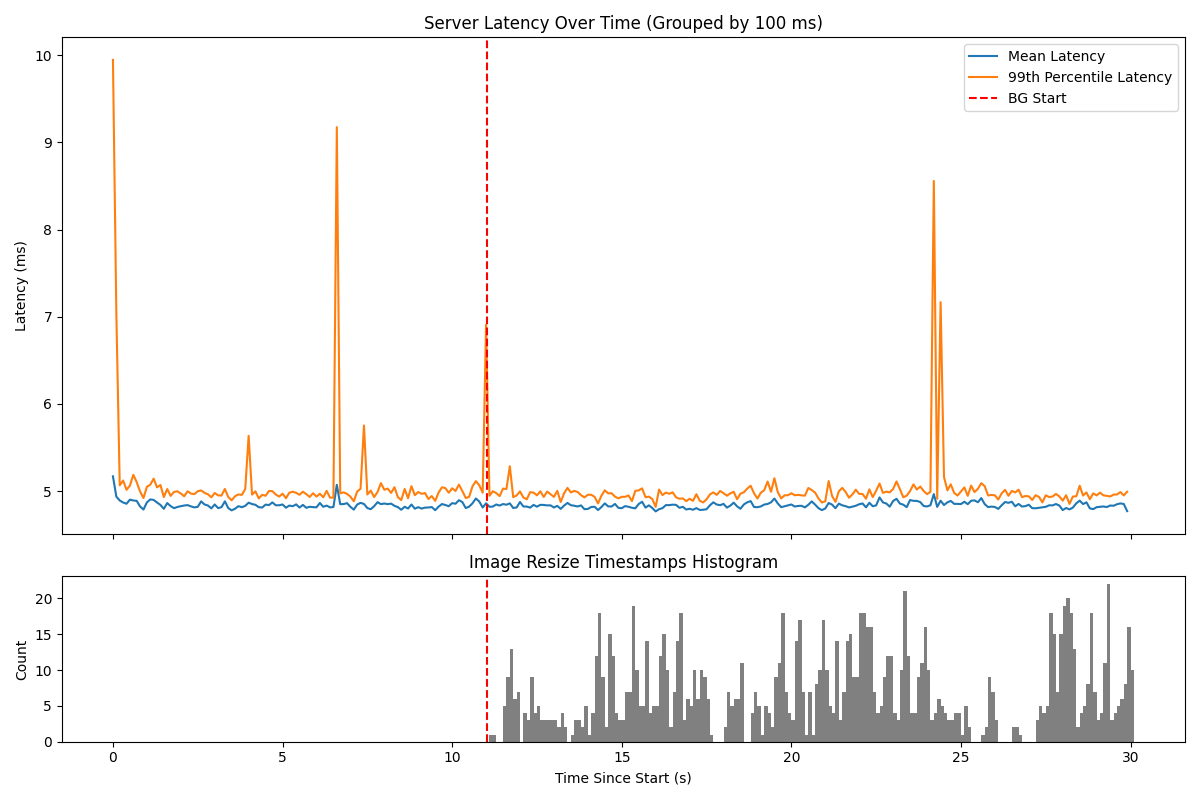
\includegraphics[width=\columnwidth]{graphs/patched-idle-low-two.png}
        \caption{Low load}\label{fig:patched-idle-low-two}
    \end{subfigure}
    \hspace{\fill}
    \begin{subfigure}[t]{0.49\columnwidth}
        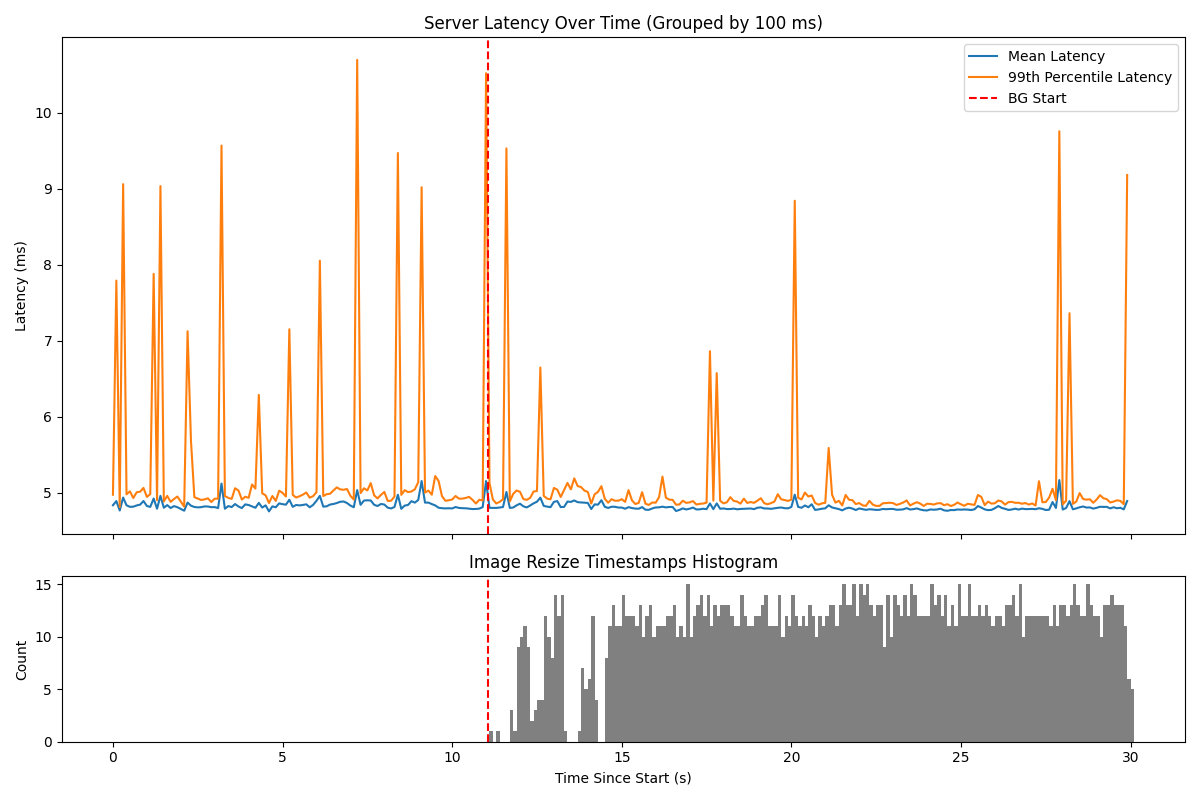
\includegraphics[width=\columnwidth]{graphs/patched-idle-high-two.png}
        \caption{High load}\label{fig:patched-idle-high-two}
    \end{subfigure}
    \vspace{4pt}
    \caption{using a patched \schedidle{} that steals queued \schednormal{}
    tasks before running \schedidle{} ones}\label{fig:patched-idle}
\end{figure}

\begin{figure}[t]
    \centering
    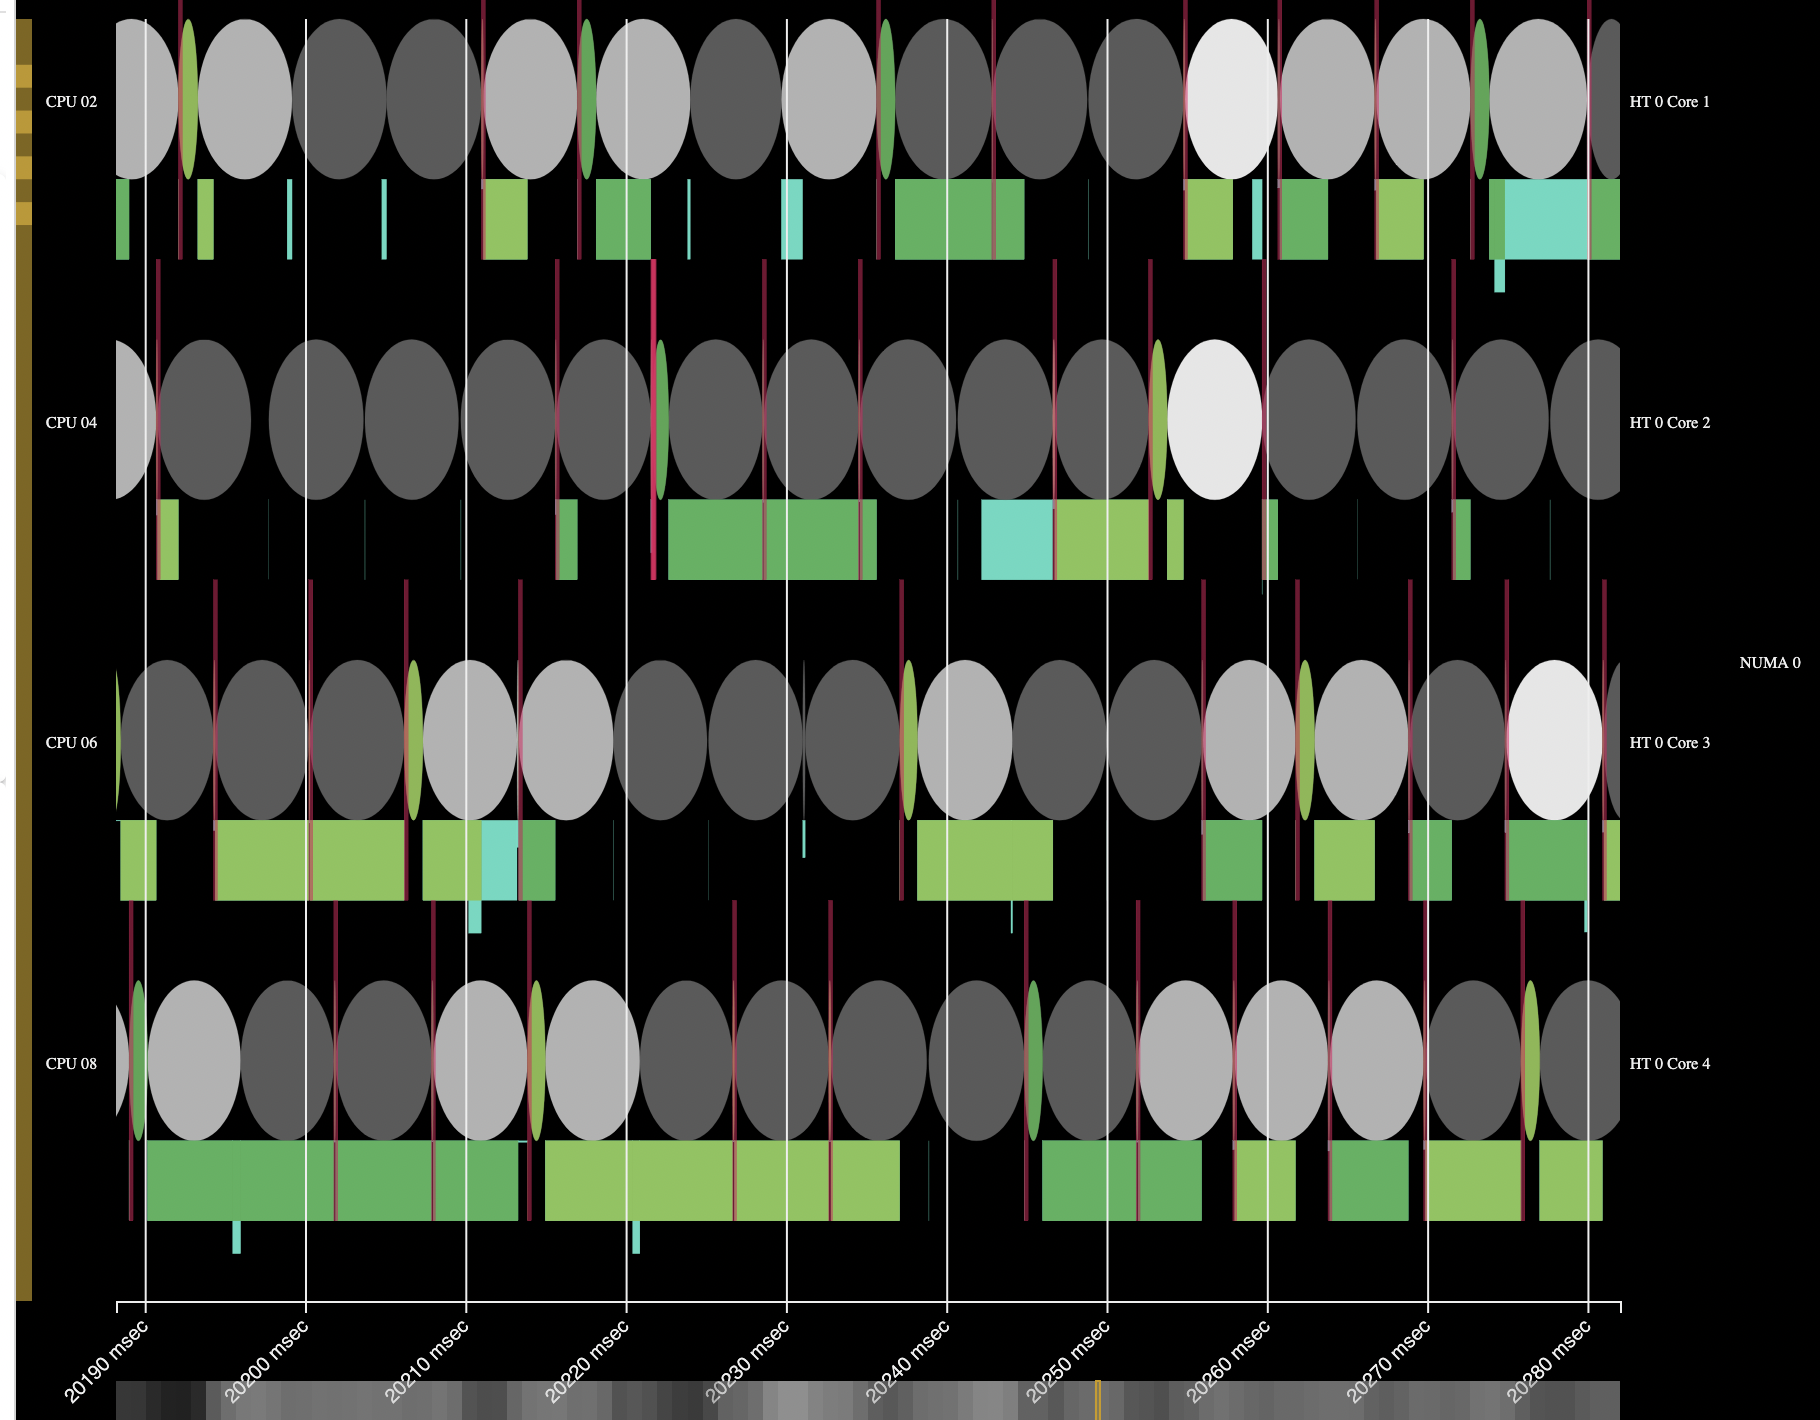
\includegraphics[width=\columnwidth]{graphs/schedviz-patched.png}
    \caption{The BE threads are colored in two different shades of green, the LC
    threads are the grey ones, the red vertical lines are the scheduler
    initially choosing a BE thread, which leads to an attempt to steal a queued
    LC one. As a result, BE threads only run when there are no queued LC
    threads.}\label{fig:schedviz-patched}
\end{figure}

This work focuses on cpu allocation, and thus will show the strongest gains for
applications that are cpu bound. 

We test the patch in two different settings: the cpu-bound example server we
have been using for the graphs in this paper so far, and an example web application
that we run using Kubernetes, that uses a mix of i/o and cpu.

For the experiment we have used throughout the paper, we set the BE workloads to
be marked as idle via the \cgroups{} api. We can see the resulting performance
in \autoref{fig:patched-idle}. As desired the latency of the server remains
stable after the background tasks start. This does not mean that the background
task never runs: the lower graph still shows iterations of image resizing being
done. The difference is that now the background tasks will reliably get
interrupted when the LC server has a request to process. We can see this
happening in an outtake of the schedviz visualization for one of the runs in
\autoref{fig:schedviz-patched}. The green BE processes only run in the gaps
where there is no queued LC process, and are immediately preempted when one
wakes up, on whatever core that may be. The red lines show when the core has
chosen intially to run a BE process, sometimes followed by an LC process that
was stolen as a result running next, sometimes by the BE process actually
running because there was no queued LC thread to steal.

For the web application, we build a REST-api on top of FastAPI, and deploy it
using async gunicorn workers. The web application itself is a recommendation
service, it has a connection to a database, which is makes requests to and
processes data from.



% \subsection{Verifying patch behavior}

% \begin{figure}[t]
%     \centering
%     \begin{subfigure}[t]{0.49\columnwidth}
%         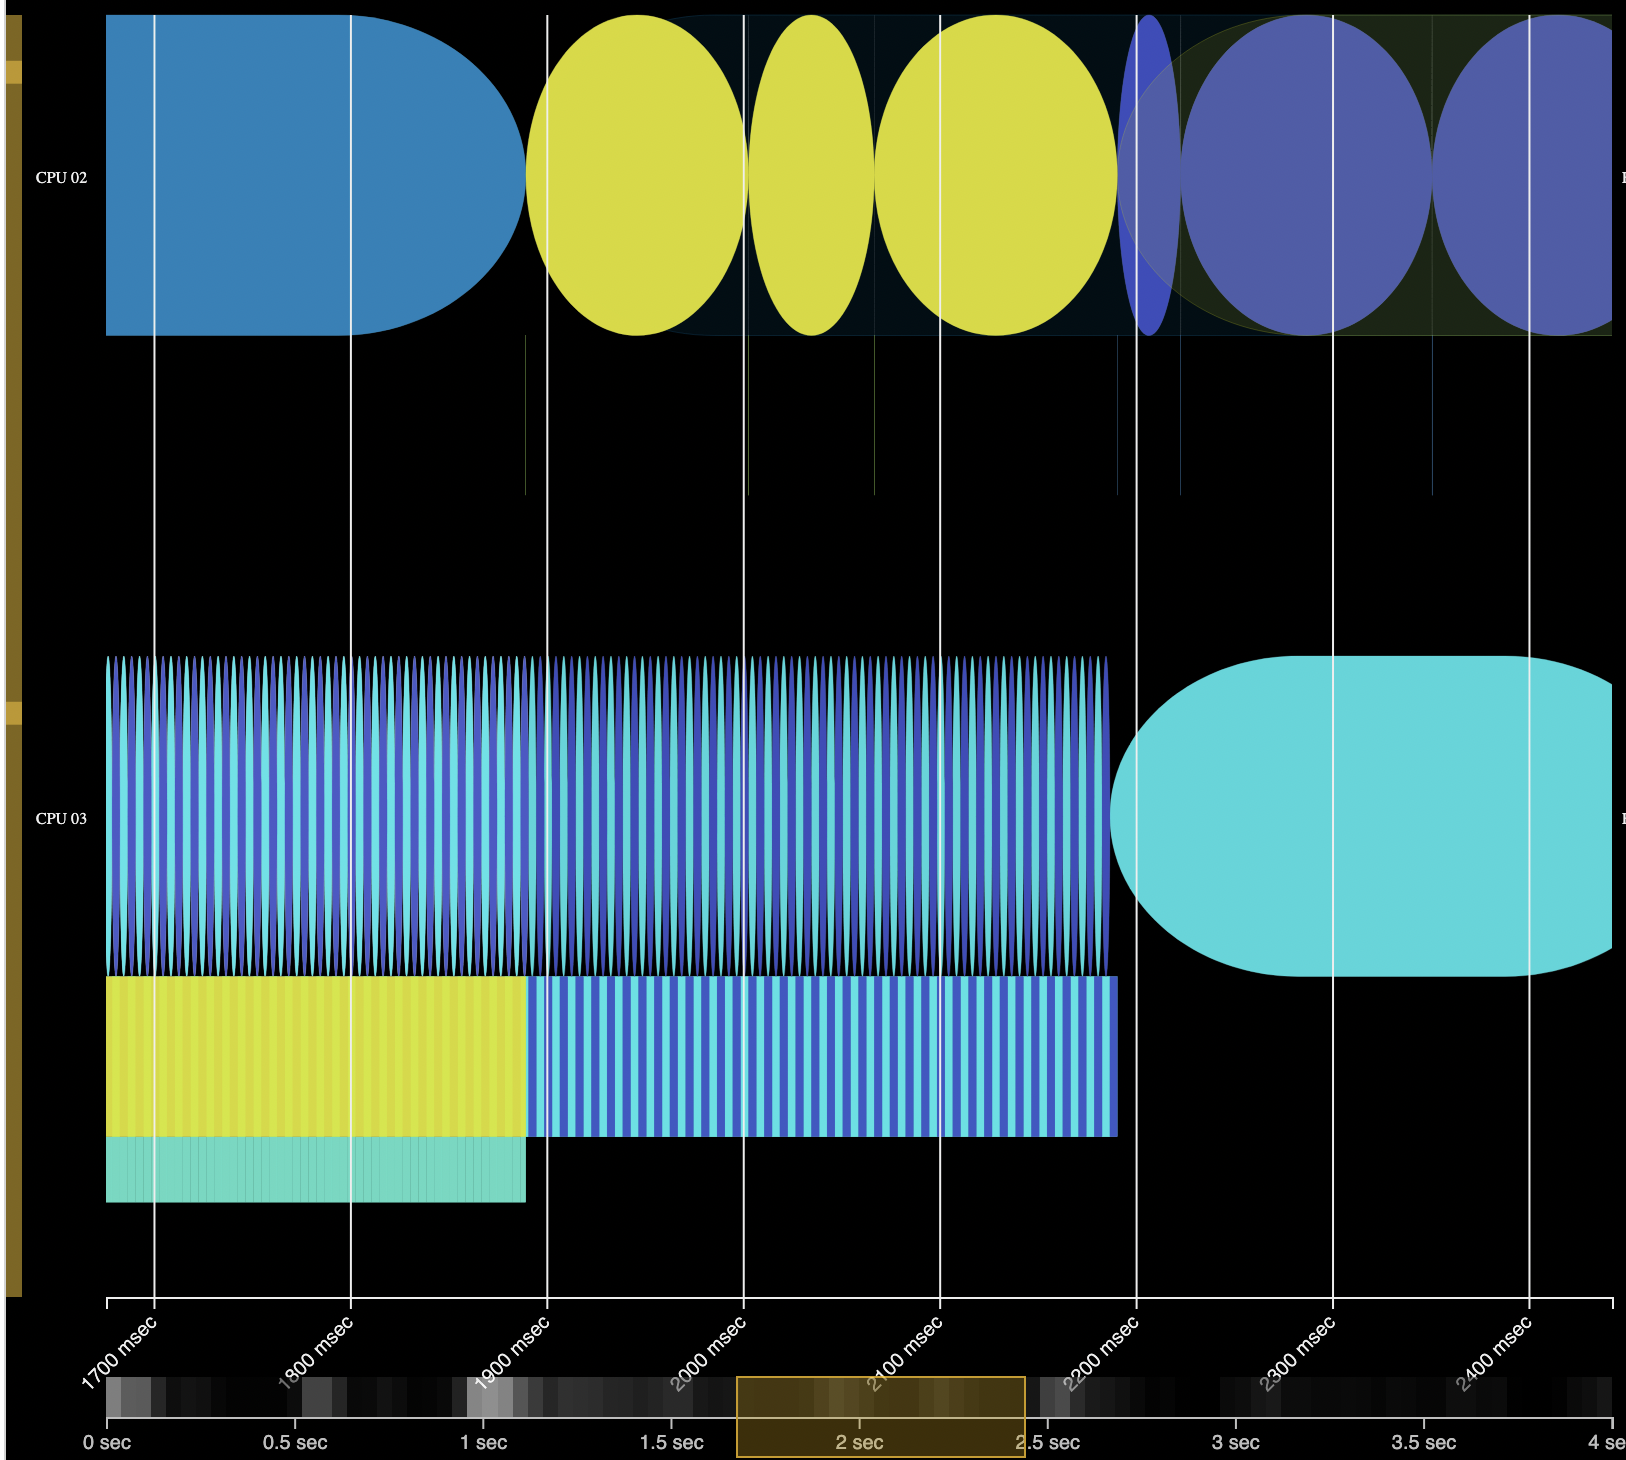
\includegraphics[width=\columnwidth]{graphs/schedviz-steal-unedited.png}
%         \caption{unedited Linux}
%     \end{subfigure}
%     \hspace{\fill}
%     \begin{subfigure}[t]{0.49\columnwidth}
%         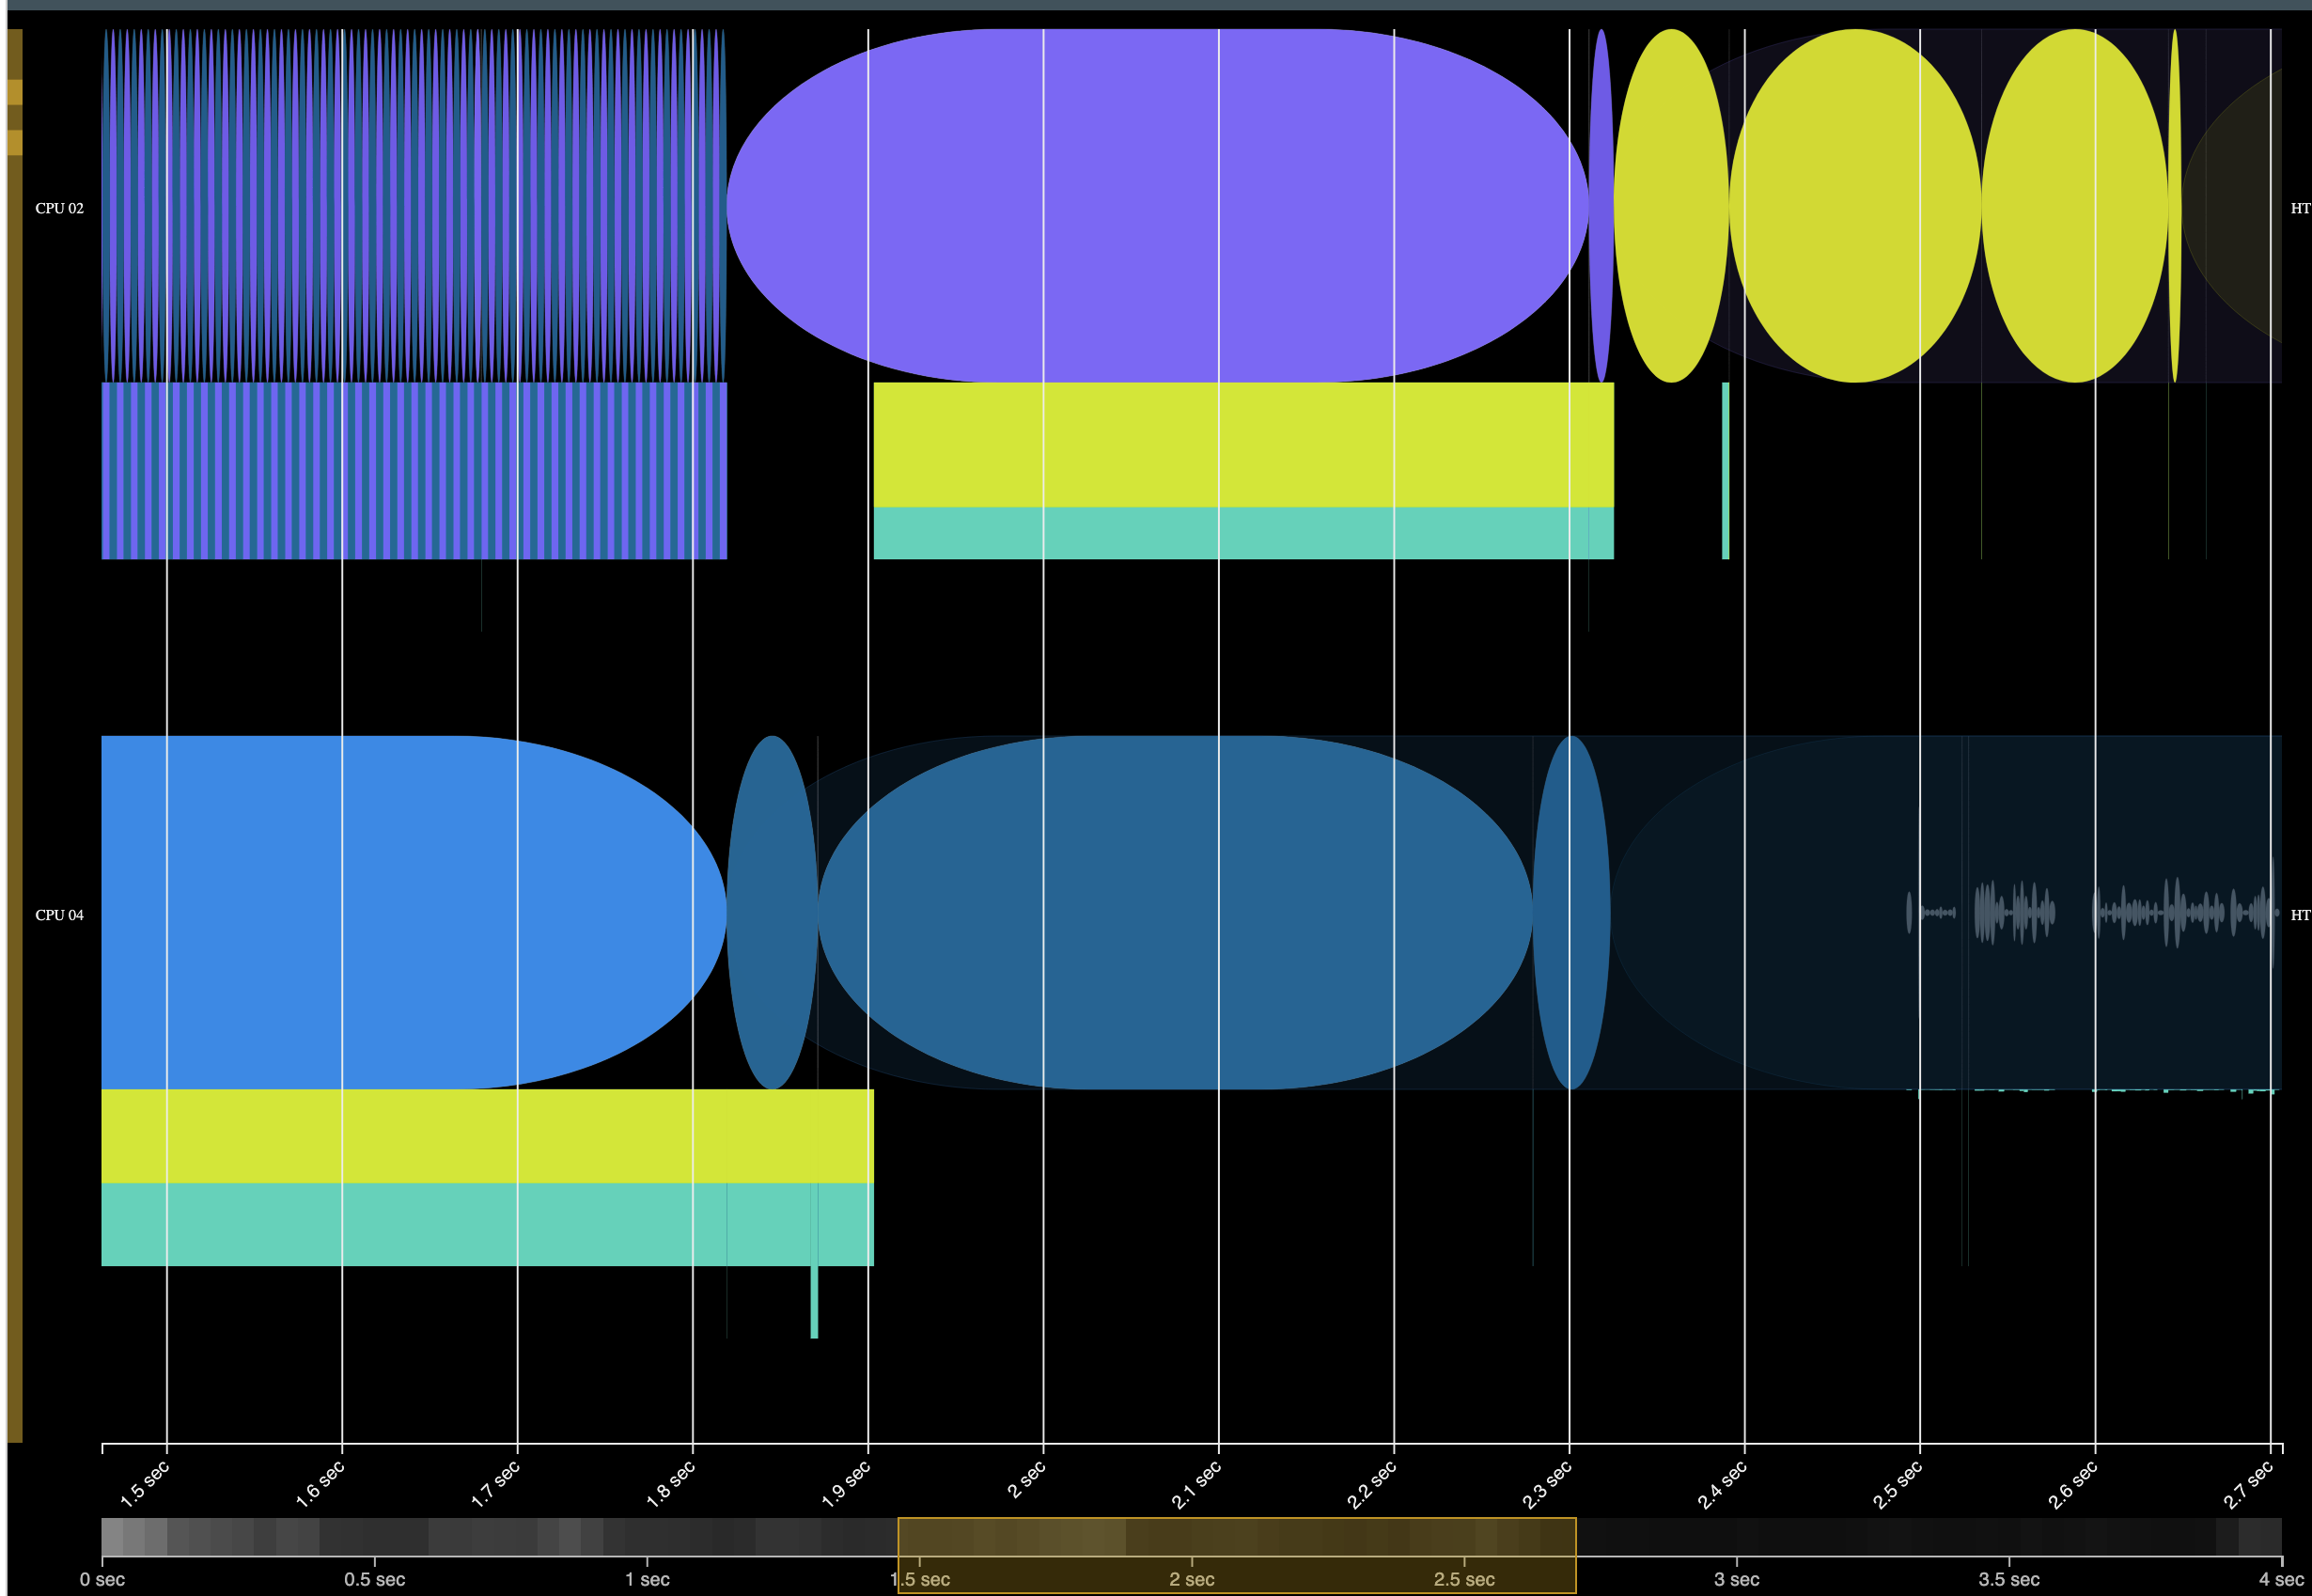
\includegraphics[width=\columnwidth]{graphs/schedviz-steal-patched.png}
%         \caption{patched Linux}
%     \end{subfigure}
%     \vspace{4pt}
%     \caption{microbench on two cores; in both diagrams the different shades of blue are the
%     \schednormal{} processes and the yellow is the \schedidle{} process}\label{fig:steal-micro}
% \end{figure}

% We begin by looking at the behavior of the patch in a microbenchmark. On three
% cores, we run two \schednormal{} processes and one \schedidle{} process. We
% visualize the scheduling decisions made by both an unedited and patched version
% of the kernel in \autoref{fig:steal-micro}. We observe that the scheduler
% initially runs two of the \schednormal{} processes on one core and the third on
% the other core. When the latter finishes, the unedited version of Linux will run
% the \schedidle{} process on that core; whereas the patched version will steal
% the queued \schednormal{} process from the other core. 

% We conclude that the patch works as expected, and is able to enforce the
% categorical separation of \schednormal{}, ie LC, and \schedidle{}, ie BE,
% workloads across cores.